\documentclass[../monografia.tex]{subfiles}

\begin{document}
\section{Arquitetura da Rede}

\subsection{Conexão de Dispositivos}
Como citado anteriormente, as medições realizadas pelos dispositivos precisam ser salvas e enviadas para algum local de armazenamento, para posterior análise, exigindo que seja estabelecido um protocolo de conexão. Com o crescimento do conceito de Internet das Coisas, novas tecnologias para conexão rápida, segura e fácil de dispositivos surgem.

Wi-Fi é uma família de tecnologias designadas para comunicação sem fio baseada no padrão IEEE 802.11, amplamente utilizada em redes de área local (em inglês \textit{local area network}, LAN) para prover acesso à internet. Essa tecnologia opera nas faixas de 2,4 e 5GHz, sendo que a primeira permite uma taxa de transmissão de até 600 Mbits/s e a segunda até 1 Gbit/s em casos mais extremos \cite{Wi-Fi-datarate}. Em contrapartida, possui a desvantagem de só funcionar bem em distâncias relativamente pequenas e possui um consumo de energia elevado.

Uma outra tecnologia para comunicação sem fio amplamente utilizada hoje em dia é o Bluetooth, que surgiu com objetivo inicial substituir a conexão por fios entre dispositivos, porém já evoluiu muito e é encontrada em diversas aplicações. Em 2017, a \textit{Bluetooth Special Interest Group} (Bluetooth SIG, organização que gerencia o desenvolvimento do padrão Bluetooth) definiu uma arquitetura de rede em malha baseada na versão de baixo consumo de energia \textit{Bluetooth Low Energy} (BLE) --- \textit{Bluetooth Mesh} \cite{BLE-mesh}, uma rede de área pessoal sem fio (WPAN), que permite o estabelecimento de uma comunicação \textit{many-to-many} entre os dispositivos da rede. Essa arquitetura utiliza o conceito de rede por inundação, no qual os dados de um nó são enviados para vários outros nós, que atuam como retransmissores desses dados para outros dispositivos dentro do seu alcance, o que aumenta a área de cobertura da rede além do limite de comunicação 1 para 1, com limite de 32 mil nós em uma só rede. Os dispositivos da rede podem ser heterogêneos, possuindo diferentes funções. A tecnologia BLE foi desenvolvida exatamente para aplicações onde é necessário um baixo consumo de energia, o que impõe um limite na sua taxa de transmissão de dados.

Dados os requisitos desse projeto, os dispositivos serão interconectados por meio de uma rede \textit{Bluetooth Mesh}, disponibilizando dados de medições dos sensores e \textit{feedback} ao longo do dia por toda a rede. Como estamos utilizando um dispositivo com conectividade tanto Bluetooth quanto Wi-Fi, um dos dispositivos da rede estará conectado também à internet via Wi-Fi, para que seja possível enviar os dados coletados pela rede para um banco de dados localizado em um servidor externo ao sistema, possibilitando o acesso remoto aos dados.

\begin{figure}[h!]
    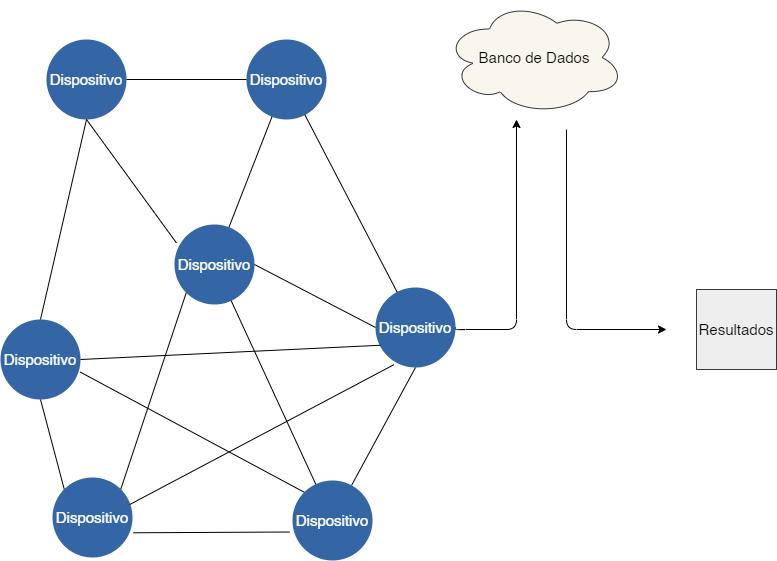
\includegraphics[width=\textwidth]{arq_rede}
    \caption{Arquitetura da rede de dispositivos}
    \label{fig:Diagrama de Blocos}
\end{figure}

\subsection{Banco de Dados}
Outro requisito comumente encontrado em dispositivos IoT focados em monitoramento é a alta disponibilidade de dados para que esse monitoramento em questão seja realizado de forma eficiente. Isso faz com que soluções de armazenamento em nuvem sejam boas alternativas, já que os dados estariam armazenados em um servidor externo ao sistema, possibilitando o seu acesso remotamente. Grandes empresas de tecnologia oferecem plataformas de desenvolvimento com interfaces de programação de aplicações (API, do inglês \textit{application programming interface}) que facilitam o desenvolvimento de bancos de dados conectados.

Para esse projeto, usaremos a solução AWS da Amazon, especificamente o serviço \textbf{AWS IoT Core} \cite{aws-iot}, que é um serviço que permite conexão de dispositivos a aplicativos em nuvem. Ele será utilizado em conjunto com o banco de dados NoSQL DynamoDB da própria plataforma.


\section{Arquitetura do Dispositivo} % Como atingir os objetivos (requisitos) e apronfunda specs da descrição do problema (especificação inicial)

\begin{figure}[h!]
    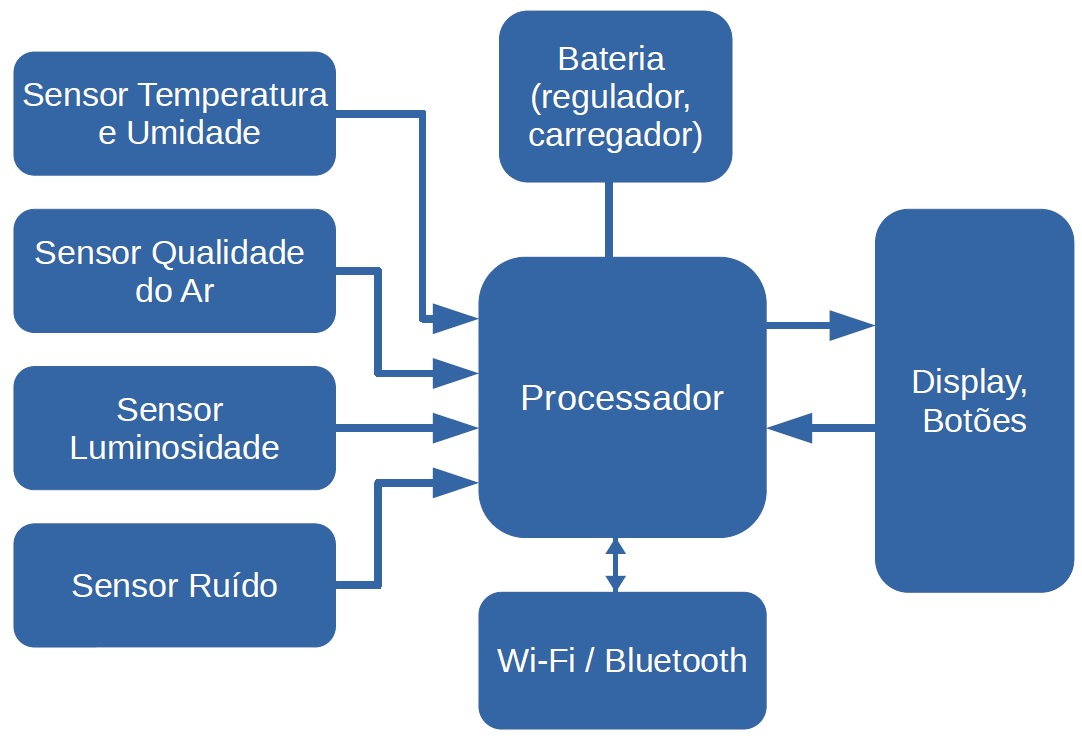
\includegraphics[width=\textwidth]{block_diagram}
    \caption{Diagrama de Blocos do Hardware do Dispositivo}
    \label{fig:Diagrama de Blocos}
\end{figure}

\subsection{\textit{Processador}}

De acordo com a pesquisa de 2019 da Aspencore \cite{eetimes}, 61\% dos projetos de sistemas embarcados usam processadores de 32-bits, e 65\% utiliza algum tipo de sistema operacional. 

A partir disso e listando os periféricos necessários para comunicação com os periféricos (descritos a seguir), selecionamos as principais opções existentes no mercado de microcontroladores para atuar como processador central do dispositivo. 

Como existem a comunicação dos dispositivos é uma funcionalidade crucial, juntamos opções de \textit{System-on-a-Chip} (SoC), ou Sistema em um chip, que trata-se de um circuito integrado que engloba processadores (ou microcontroladores, em dispositivos embarcados), memórias, dentre outros módulos, como circuitos para comunicação sem fio, personalizados para uma aplicação \cite{soc}. 

\begin{center}
\begin{tabular}{|c|c|c|c|c|} 
\hline
\textbf{Vendor} & \textbf{Chip} & \textbf{Price} & \textbf{Kit} & \textbf{Kit Price} \\
\hline
Nordic Semi & BMD350 & \$11.3 & BMD350-EVAL & \$89 \\ 
Espressif Systems & ESP32 & \$3.8 & ESP32-DevKitC & \$10 \\ 
STMicroelectronics & BlueNRG-2 & \$3.5 & BlueNRG-Tile & \$50 \\ 
\hline
\end{tabular}
\end{center}

Para decidir entre as três opções apresentadas, analisamos principalmente os ambientes de desenvolvimento, a documentação disponível e o preço dos CIs e seus kits de desenvolvimento. 

Tendo isso em vista, escolhemos usar ESP32 \cite{ESP32}, que é uma família de \textit{SoC}s da fabricante Espressif que possui um microcontrolador integrado às tecnologias Wi-Fi e Bluetooth. Por ter um bom suporte e ferramentas de desenvolvimento focadas em BLE e Wi-Fi, além de ter um dos menores preços, foi nossa escolha como melhor custo-benefício. 

\textbf{Especificações do ESP32:} \cite{ESP-datasheet}
\begin{itemize}
\item \textbf{Processador}: Xtensa 32-bits, dual core
\item \textbf{Wi-Fi}: 802.11 b/g/n
\item \textbf{Bluetooth}: v4.2 BR/EDR e BLE
\end{itemize}


\subsection{Sensores}
A fim de atender aos critérios apresentados para o monitoramento, foram escolhidos os seguintes sensores: 
\begin{itemize}
\item \textbf{AS7262}\cite{as7262}, da AMS: 

Atende aos requisitos de medição de \textit{conforto luminoso}. 

\textbf{Medidas}: Intensidade e cor da luz incidente.

A cor da luz, nesse sensor, é medida através de 6 canais, correspondendo aos espectros de luz vermelha (650nm), laranja (600nm), amarela (570nm), verde (550nm), azul (500nm) e violeta (450nm), ao invés de simples RGB, com resolução de 16 bits.

\textbf{Comunicação}: I²C, SPI ou UART (configurável)

\item \textbf{BME280} \cite{bme280}, da Bosch: 

Atende aos requisitos de \textit{conforto térmico}. 

\textbf{Medidas}: 
    \begin{itemize}
    \item Temperatura entre -40 e 85ºC, com precisão de ±1.0°C
    \item Umidade relativa com precisão de ±3\%
    \item Pressão entre 300 e 1100hPa, com precisão ±1 hPa
    \end{itemize}

\textbf{Comunicação}: SPI ou I²C

\item \textbf{SGP30} \cite{sgp30}:

Sensor para medições de aplicação \textit{indoor}. 

\textbf{Medidas}:
    \begin{itemize}
    \item TVOC entre 0 ppb e 60000 ppb, com resolução de 1ppb
    \item $CO_{2}$ entre 400 ppm e 60000 ppm, com resolução de 1ppb
    \end{itemize}

\textbf{Comunicação}: I²C

\item \textbf{Microfone de Eletreto}:

Em conjunto com um circuito amplificador, atende aos requisitos de \textit{conforto acústico}. 

\textbf{Medida}: volume de ruído sonoro ambiente

\textbf{Comunicação}: Analógica, precisão de 12 bits (resolução do conversor analógico-digital do ESP32). 
\end{itemize}

\subsection{Sistema de coleta de Feedback}

Para a coleta do \textit{feedback} nos dispositivos, optamos por utilizar um display e 2 botões. 

\subsection{Alimentação}

Para alimentar os dispositivos, foi pensado em utilizar uma bateria de Lítio-Polímero, de uma célula (1S), por ter a maior densidade energética dentre as baterias recarregáveis, permitindo que o dispositivo seja portátil e não dependente da rede elétrica. A capacidade da bateria será definida com base nos testes de consumo do equipamento nas etapas finais de desenvolvimento do protótipo. 

A bateria LiPo tem tensões de operação entre 3.5 e 4.2 Volts. Para alimentar o circuito foi optado por elevar a tensão para 5V, através de um regulador chaveado boost, ainda não definido. 

Para fazer a recarga da bateria de forma eficiente e segura, foi pensado em um circuito carregador utilizando o CI TP4056 \cite{tp4056}, alimentado por 5V através de um conector USB-micro. Com esse CI é possível também que o circuito opere enquanto a bateria está sendo recarregada. 


\end{document}
